\begin{equation}
    \begin{gathered}
        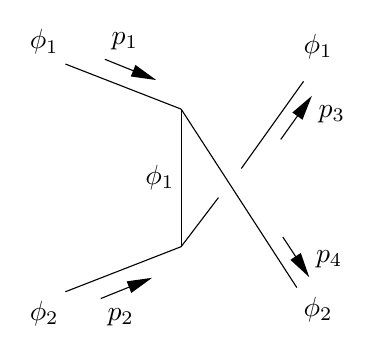
\begin{tikzpicture}[x=0.75pt,y=0.75pt,yscale=-1,xscale=1]
            %uncomment if require: \path (0,300); %set diagram left start at 0, and has height of 300
            
            %Straight Lines [id:da3426510440775925] 
            \draw    (248.45,195.45) -- (192.71,109.45) ;
            %Straight Lines [id:da5923518951291684] 
            \draw    (136.97,87.74) -- (192.71,109.45) ;
            %Straight Lines [id:da8812815107092951] 
            \draw    (155.98,85.45) -- (178.85,94.7) ;
            \draw [shift={(180.71,95.45)}, rotate = 202.02] [fill={rgb, 255:red, 0; green, 0; blue, 0 }  ][line width=0.08]  [draw opacity=0] (12,-3) -- (0,0) -- (12,3) -- cycle    ;
            %Straight Lines [id:da30564429983765695] 
            \draw    (254.54,104.69) -- (240.71,124.07) ;
            \draw [shift={(255.71,103.07)}, rotate = 125.54] [fill={rgb, 255:red, 0; green, 0; blue, 0 }  ][line width=0.08]  [draw opacity=0] (12,-3) -- (0,0) -- (12,3) -- cycle    ;
            %Straight Lines [id:da6306489775151924] 
            \draw    (192.71,109.45) -- (192.71,175.74) ;
            %Straight Lines [id:da668839367321165] 
            \draw    (210.71,152.07) -- (192.71,175.74) ;
            %Straight Lines [id:da1836661274128617] 
            \draw    (136.97,197.45) -- (192.71,175.74) ;
            %Straight Lines [id:da7473359384686846] 
            \draw    (153.98,200.74) -- (176.85,191.49) ;
            \draw [shift={(178.71,190.74)}, rotate = 517.98] [fill={rgb, 255:red, 0; green, 0; blue, 0 }  ][line width=0.08]  [draw opacity=0] (12,-3) -- (0,0) -- (12,3) -- cycle    ;
            %Straight Lines [id:da5965521376969758] 
            \draw    (253.35,188.78) -- (241.71,171.07) ;
            \draw [shift={(254.45,190.45)}, rotate = 236.68] [fill={rgb, 255:red, 0; green, 0; blue, 0 }  ][line width=0.08]  [draw opacity=0] (12,-3) -- (0,0) -- (12,3) -- cycle    ;
            %Straight Lines [id:da6225912631978587] 
            \draw    (251.71,96.07) -- (246.17,103.82) -- (221.71,138.07) ;
            
            % Text Node
            \draw (134.97,84.34) node [anchor=south east] [inner sep=0.75pt]    {$\phi _{1}$};
            % Text Node
            \draw (134.97,200.85) node [anchor=north east] [inner sep=0.75pt]    {$\phi _{2}$};
            % Text Node
            \draw (157.98,82.05) node [anchor=south west] [inner sep=0.75pt]    {$p_{1}$};
            % Text Node
            \draw (155.98,204.14) node [anchor=north west][inner sep=0.75pt]    {$p_{2}$};
            % Text Node
            \draw (190.71,142.59) node [anchor=east] [inner sep=0.75pt]    {$\phi _{1}$};
            % Text Node
            \draw (257.71,106.47) node [anchor=north west][inner sep=0.75pt]    {$p_{3}$};
            % Text Node
            \draw (256.45,187.05) node [anchor=south west] [inner sep=0.75pt]    {$p_{4}$};
            % Text Node
            \draw (250.45,86.34) node [anchor=south west] [inner sep=0.75pt]    {$\phi _{1}$};
            % Text Node
            \draw (250.45,198.85) node [anchor=north west][inner sep=0.75pt]    {$\phi _{2}$};
            \end{tikzpicture}            
    \end{gathered} \eqqcolon \ii \mathcal{M}_{u1} = \frac{\ii}{(p_1 - p_4)^2 + \ii 0^+} (\ii g)^2 = - \ii \frac{g^2}{u + \ii 0^+}.
\end{equation}